%% Autor: Björn Ritterbecks 
%% Letzte Aenderung: 15.06.2016 
\begin{marginfigure}
\vspace*{0.2cm}
\centering
%\sansmath
 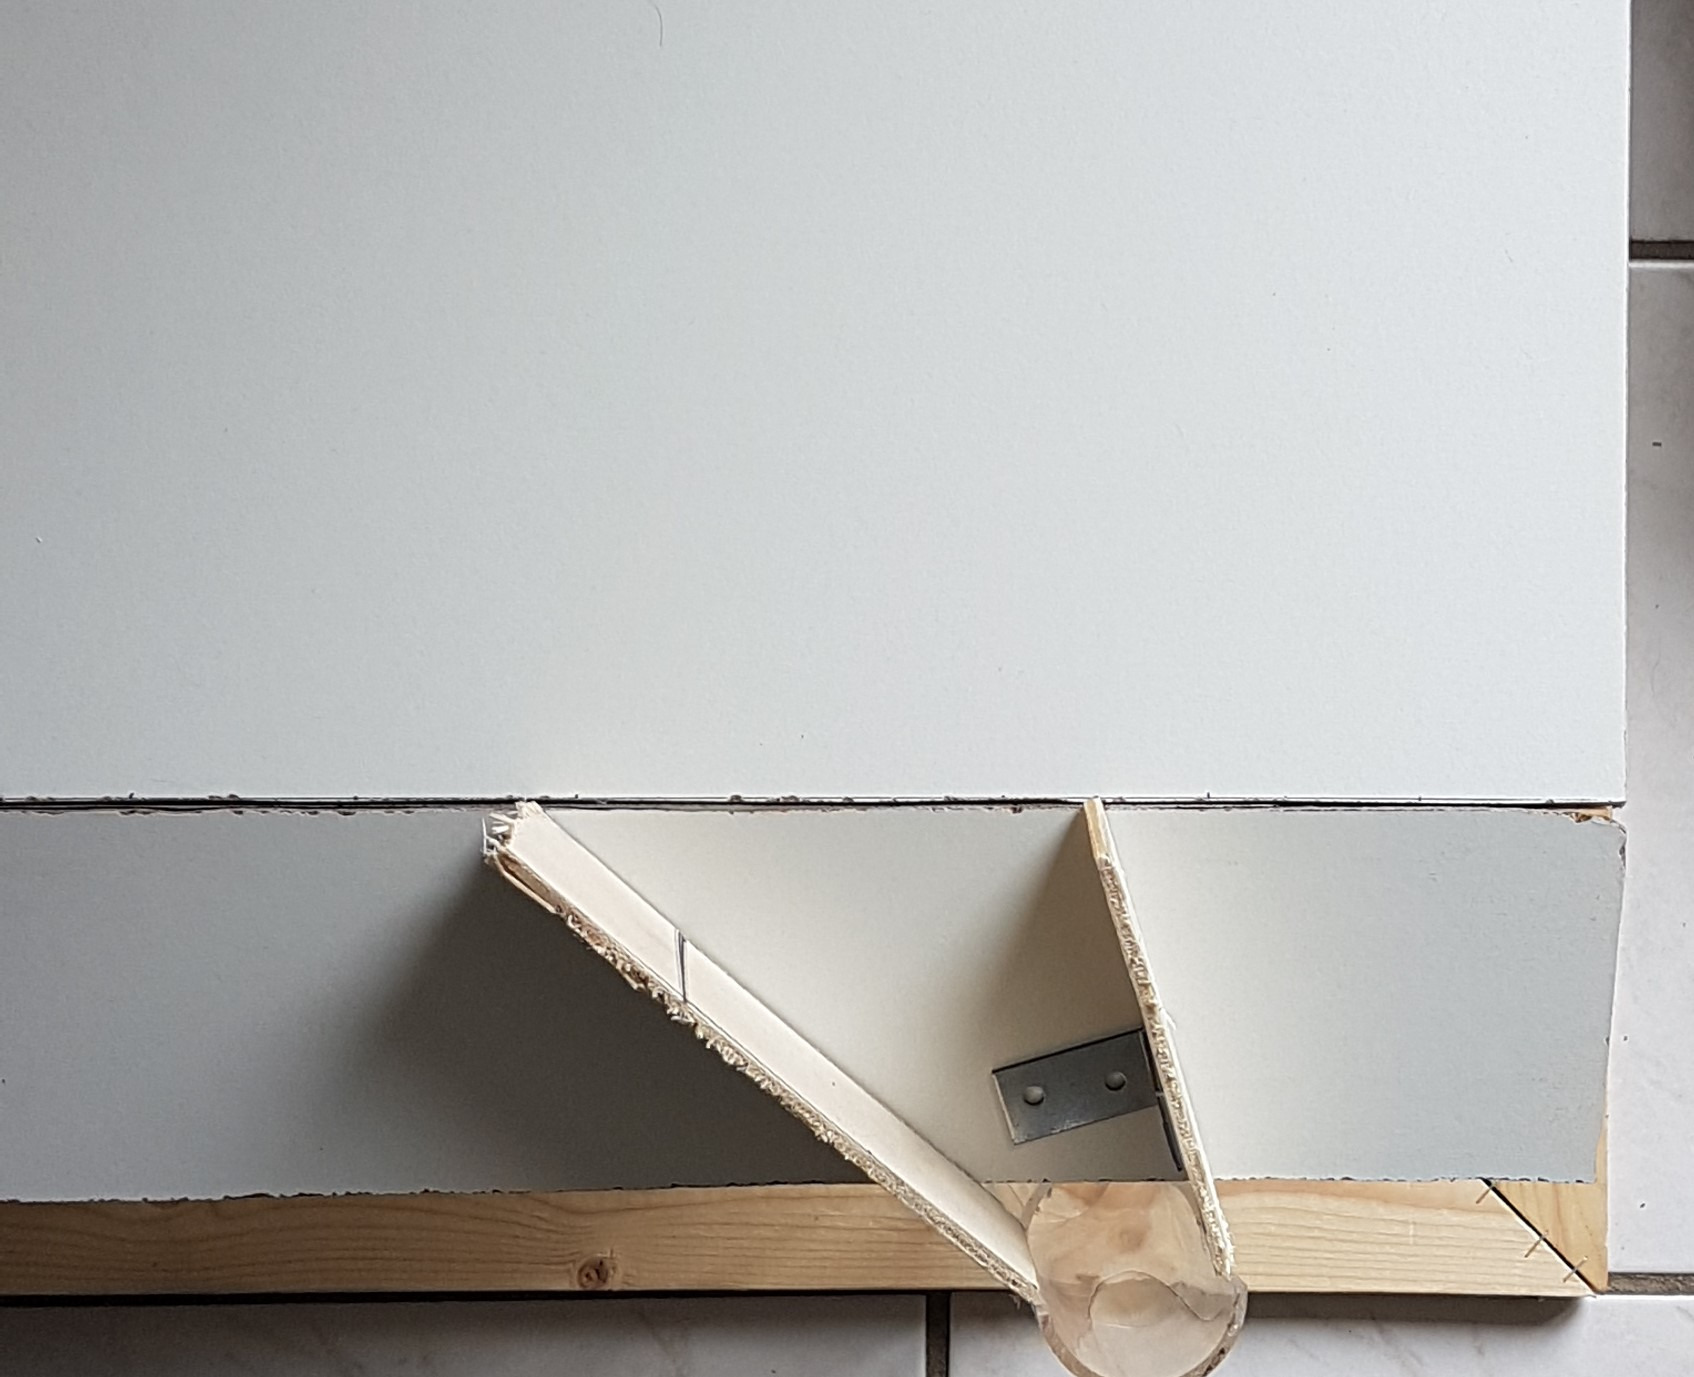
\includegraphics[width=0.99\marginparwidth]{images/istregistriert.jpg}
  \caption[Detektionsnsprinzip]{Vorschlag einer Detektoranordnung: Je geringer der Detektionswinkel ist, desto größer muss die Breite der einzelnen Detektoren sein. Damit selbst bei den größten Detektoren alle Kugeln in die Röhren rollen können, ist der rechte Teil der Platte um $\SI{15}{\degree}$ geneigt. Ein letzter Detektor wird am rechten Ende angebracht.}
  \label{fig:istregisrtiert}
  \vspace{-0pt}
\end{marginfigure}